\documentclass{beamer}
\title{Verification of Quantum Computing}
\subtitle{and the Bloch sphere representation}
\author{Chris Henson}
\institute{Drexel University}
\date{}

\usefonttheme{structuresmallcapsserif}
\usetheme[left, hideothersubsections]{PaloAlto}
\usecolortheme{seahorse}
\usepackage{amssymb}

% no ugly icons in references
\setbeamertemplate{bibliography item}{}

% bracketed footnotes
\renewcommand*{\thefootnote}{[\arabic{footnote}]}

%remove navigation 
\setbeamertemplate{navigation symbols}{}

% sidebar excluding title
\makeatletter
  \setbeamertemplate{sidebar \beamer@sidebarside}%{sidebar theme}
  {
    \beamer@tempdim=\beamer@sidebarwidth%
    \advance\beamer@tempdim by -6pt%
    \insertverticalnavigation{\beamer@sidebarwidth}%
    \vfill
    \ifx\beamer@sidebarside\beamer@lefttext%
    \else%
      \usebeamercolor{normal text}%
      \llap{\usebeamertemplate***{navigation symbols}\hskip0.1cm}%
      \vskip1pt%
    \fi%
}%
\makeatother

\nocite{*}

% Coq code highlighting

%%%%%%%%%%%%%%%%%%%%%%%%%%%

\usepackage[utf8]{inputenc}

\DeclareUnicodeCharacter{2261}{\meq}
\DeclareUnicodeCharacter{22A4}{\mtrans}
\DeclareUnicodeCharacter{2248}{$==>$}

\DeclareRobustCommand\mtrans{ $\top$ }
\DeclareRobustCommand\meq{ $\equiv$ }

\usepackage[english]{babel}

\usepackage{xcolor}
\usepackage{listingsutf8}

\lstset{
  inputencoding=utf8,
  extendedchars=true,
	basicstyle=\scriptsize,
	frame=single
}

\definecolor{dkgreen}{rgb}{0,0.6,0}
\definecolor{ltblue}{rgb}{0,0.4,0.4}
\definecolor{dkviolet}{rgb}{0.3,0,0.5}

% lstlisting coq style (inspired from a file of Assia Mahboubi)
\lstdefinelanguage{Coq}{ 
    % Anything betweeen $ becomes LaTeX math mode
    mathescape=true,
    % Comments may or not include Latex commands
    texcl=false, 
    % Vernacular commands
    morekeywords=[1]{Section, Module, End, Require, Import, Export,
        Variable, Variables, Parameter, Parameters, Axiom, Hypothesis,
        Hypotheses, Notation, Local, Tactic, Reserved, Scope, Open, Close,
        Bind, Delimit, Definition, Let, Ltac, Fixpoint, CoFixpoint, Add,
        Morphism, Relation, Implicit, Arguments, Unset, Contextual,
        Strict, Prenex, Implicits, Inductive, CoInductive, Record,
        Structure, Canonical, Coercion, Context, Class, Global, Instance,
        Program, Infix, Theorem, Lemma, Corollary, Proposition, Fact,
        Remark, Example, Proof, Goal, Save, Qed, Defined, Hint, Resolve,
        Rewrite, View, Search, Show, Print, Printing, All, Eval, Check,
        Projections, inside, outside, Def},
    % Gallina
    morekeywords=[2]{forall, exists, exists2, fun, fix, cofix, struct,
        match, with, end, as, in, return, let, if, is, then, else, for, of,
        nosimpl, when},
    % Sorts
    morekeywords=[3]{Type, Prop, Set, true, false, option},
    % Various tactics, some are std Coq subsumed by ssr, for the manual purpose
    morekeywords=[4]{pose, set, move, case, elim, apply, clear, hnf,
        intro, intros, generalize, rename, pattern, after, destruct,
        induction, using, refine, inversion, injection, rewrite, congr,
        unlock, compute, ring, field, fourier, replace, fold, unfold,
        change, cutrewrite, simpl, have, suff, wlog, suffices, without,
        loss, nat_norm, assert, cut, trivial, revert, bool_congr, nat_congr,
        symmetry, transitivity, auto, split, left, right, autorewrite},
    % Terminators
    morekeywords=[5]{by, done, exact, reflexivity, tauto, romega, omega,
        assumption, solve, contradiction, discriminate},
    % Control
    morekeywords=[6]{do, last, first, try, idtac, repeat},
    % Comments delimiters, we do turn this off for the manual
    morecomment=[s]{(*}{*)},
    % Spaces are not displayed as a special character
    showstringspaces=false,
    % String delimiters
    morestring=[b]",
    morestring=[d],
    % Size of tabulations
    tabsize=3,
    % Enables ASCII chars 128 to 255
    extendedchars=false,
    % Case sensitivity
    sensitive=true,
    % Automatic breaking of long lines
    breaklines=false,
    % Position of captions is bottom
    captionpos=b,
    % flexible columns
    columns=[l]flexible,
    % Style for (listings') identifiers
    identifierstyle={\ttfamily\color{black}},
    % Style for declaration keywords
    keywordstyle=[1]{\ttfamily\color{dkviolet}},
    % Style for gallina keywords
    keywordstyle=[2]{\ttfamily\color{dkgreen}},
    % Style for sorts keywords
    keywordstyle=[3]{\ttfamily\color{ltblue}},
    % Style for tactics keywords
%    keywordstyle=[4]{\ttfamily\color{dkblue}},
    % Style for terminators keywords
%    keywordstyle=[5]{\ttfamily\color{dkred}},
    %Style for iterators
    %keywordstyle=[6]{\ttfamily\color{dkpink}},
    % Style for strings
    stringstyle=\ttfamily,
    % Style for comments
    commentstyle={\ttfamily\color{dkgreen}},
    %moredelim=**[is][\ttfamily\color{red}]{/&}{&/},
    literate=
    {\\forall}{{\color{dkgreen}{$\forall\;$}}}1
    {\\exists}{{$\exists\;$}}1
    {<-}{{$\leftarrow\;$}}1
    {=>}{{$\Rightarrow\;$}}1
    {==}{{\code{==}\;}}1
    {==>}{{\code{==>}\;}}1
    %    {:>}{{\code{:>}\;}}1
    {->}{{$\rightarrow\;$}}1
    {<->}{{$\leftrightarrow\;$}}1
    {<==}{{$\leq\;$}}1
    {\#}{{$^\star$}}1 
    {\\o}{{$\circ\;$}}1 
    {\@}{{$\cdot$}}1 
    {\/\\}{{$\wedge\;$}}1
    {\\\/}{{$\vee\;$}}1
    {++}{{\code{++}}}1
    {~}{{\ }}1
    {\@\@}{{$@$}}1
    {\\mapsto}{{$\mapsto\;$}}1
    {\\hline}{{\rule{\linewidth}{0.5pt}}}1
    %
}[keywords,comments,strings]

%%%%%%%%%%%%%%%%%%%%%%%%%%%

\usepackage{bbm}

\begin{document}

\frame{\titlepage}

\section{Current Research/Motivation}
\begin{frame}
\frametitle{Current Research/Motivation}
\begin{itemize}
 \item proof assistants are programming languages that allow formal proofs of mathematical theorems
 \item quantum computing is a great candidate for formal verification: it is both conceptually unintuitive and practically expensive
 \item algorithms such as Grover, Shor, etc. have been formally verified in languages such as Coq, Isabelle/HOL, etc.
 \item methods for optimizing general quantum circuits can also be verified
 \item some formalization frameworks provide the ability to export to formats such as OpenQASM and provide bindings in more accessible languages like Python
\end{itemize}
\end{frame}

\section{SU(2) $\to$ SO(3)}

\begin{frame}
\frametitle{The Bloch Sphere}
\begin{itemize}
 \item Why do we expect any connection between qubits and a sphere?
 \item In a sense the relationship between a qubit and a complex number
	 		 is the same as complex and real numbers
\end{itemize}

\begin{figure}
		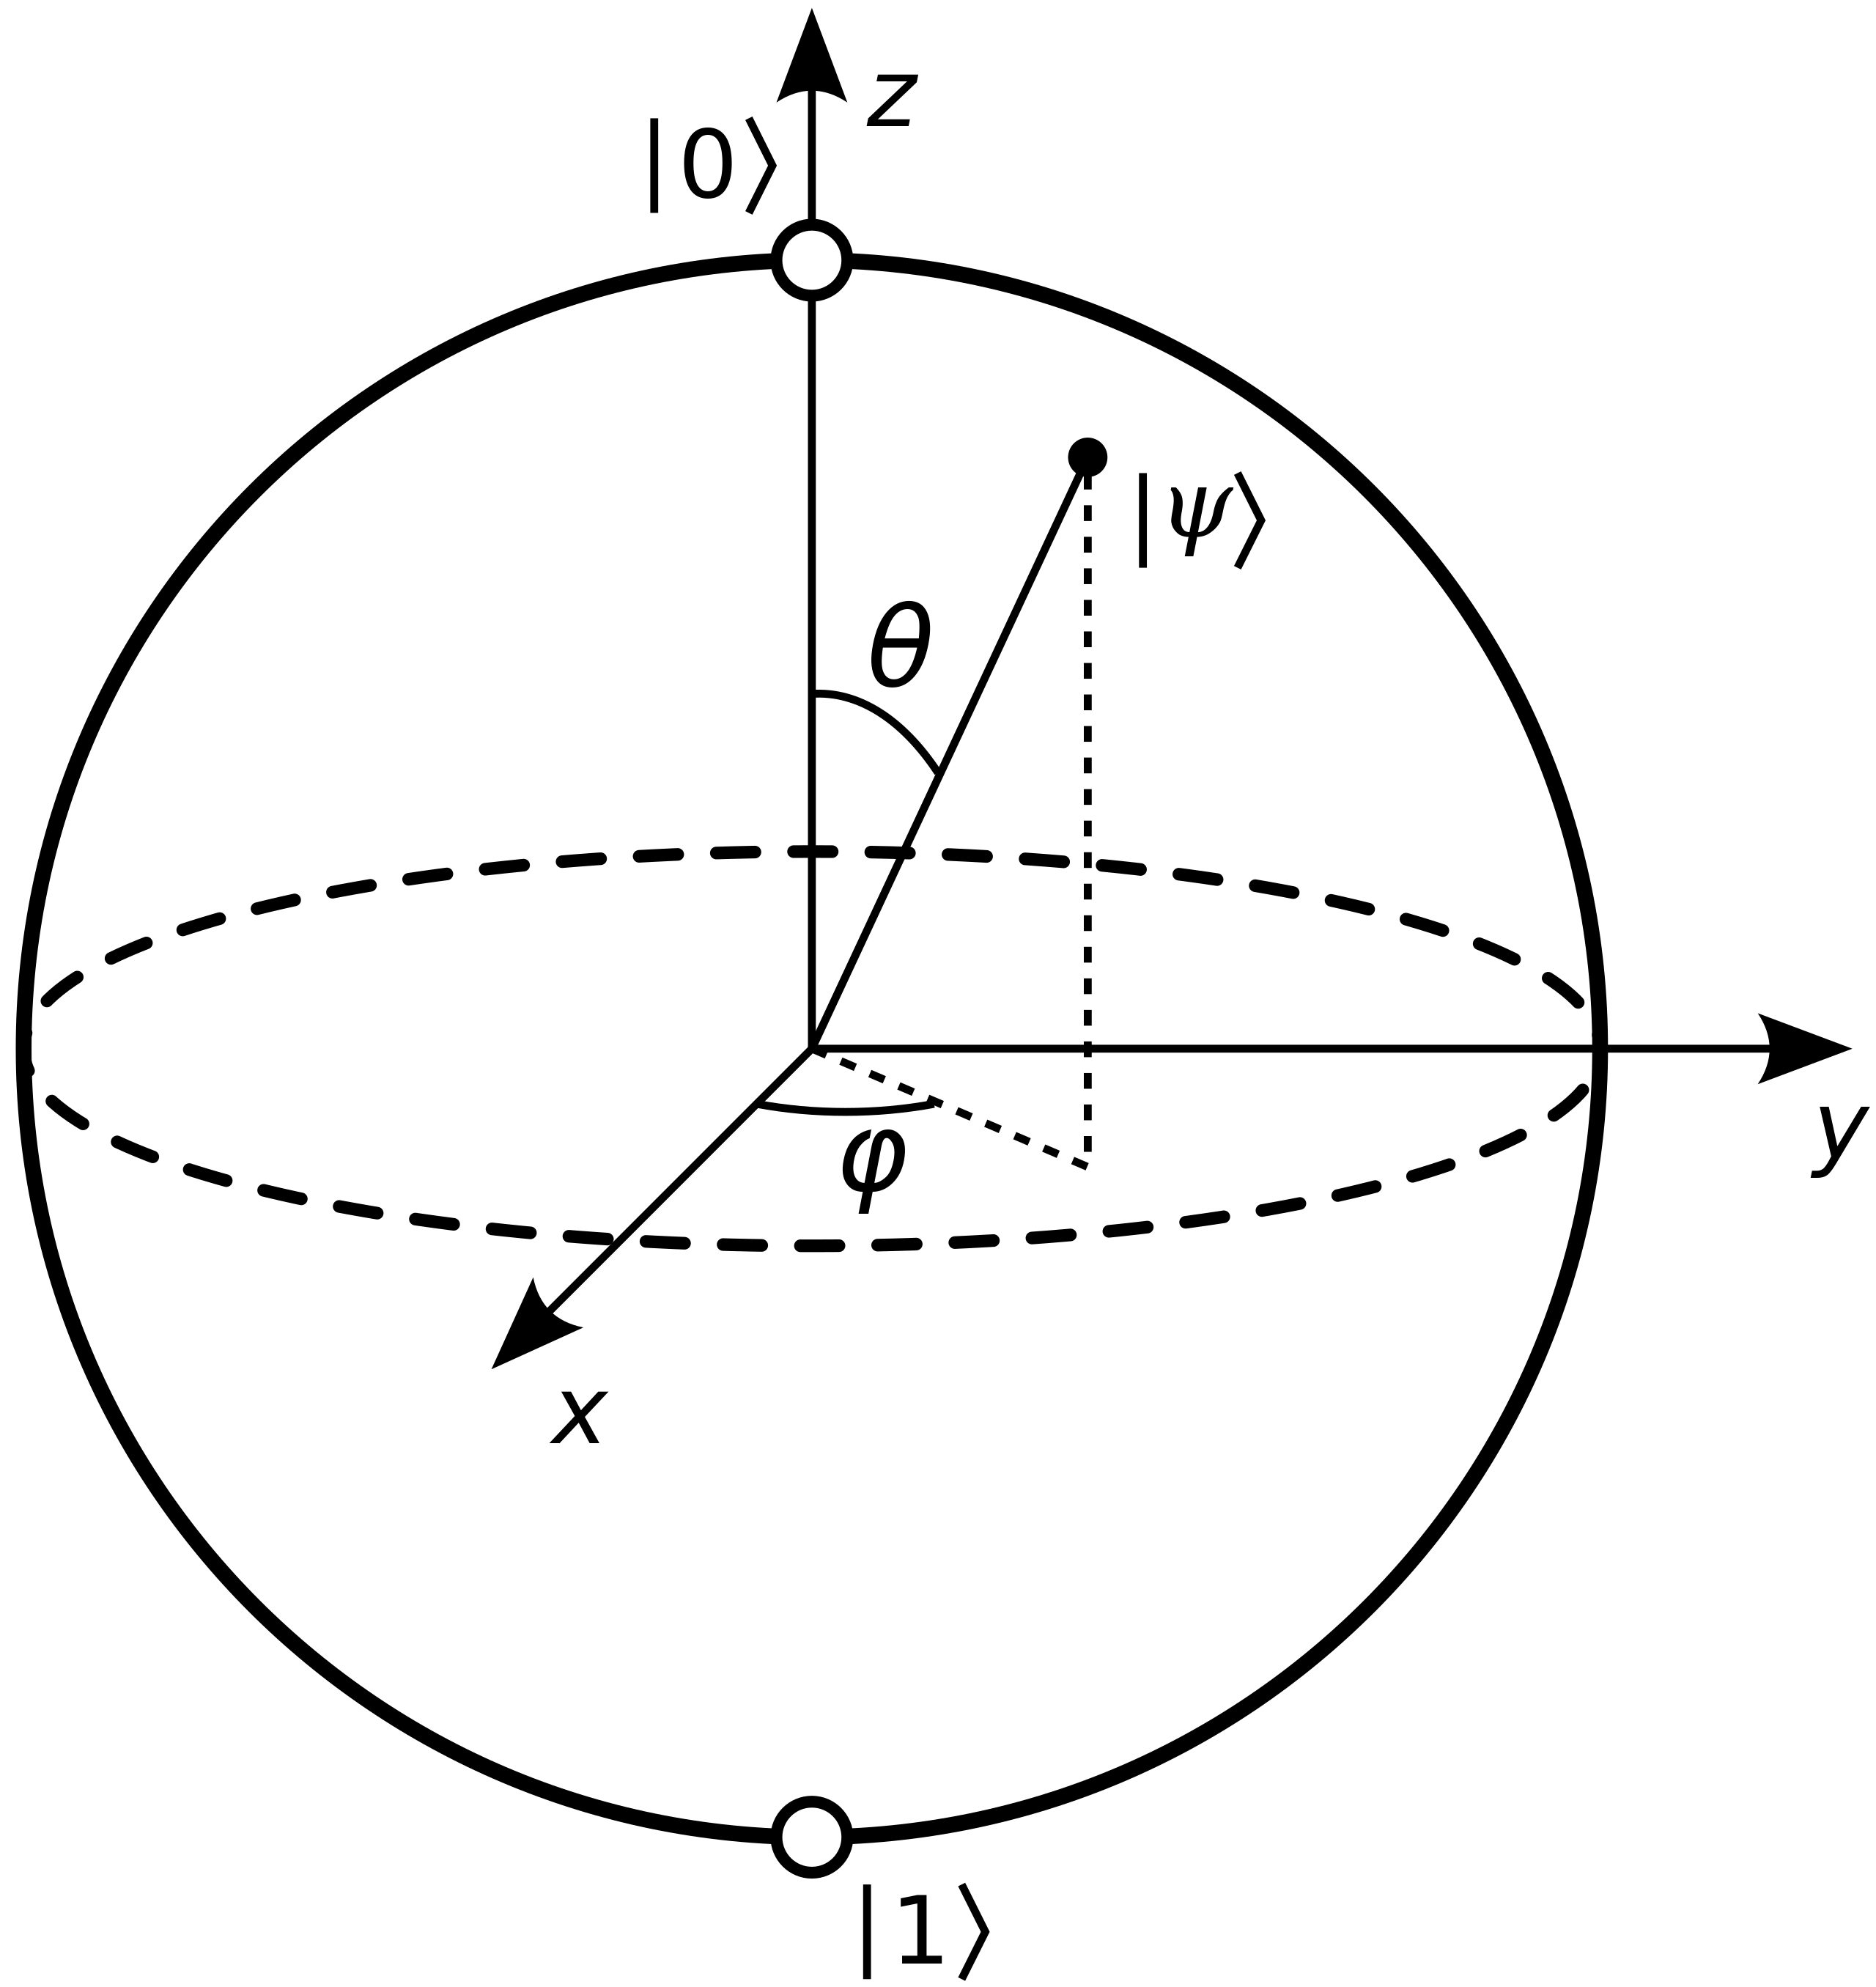
\includegraphics[width=4cm]{Bloch_sphere}
    \caption{Bloch sphere representation of a Qubit}
\end{figure}

\end{frame}

\begin{frame}
\frametitle{Groups}
\begin{definition}[Groups]
A group is a set $G$ with operation $\cdot$, such that:

\begin{itemize}
	\item $\forall a, b \in G: a \cdot b \in G$
	\item $\forall a, b, c \in G: (a \cdot b) \cdot c = a \cdot (b \cdot c)$
	\item $\forall a \in G, \exists \mathbbm{1} \in G: a \cdot \mathbbm{1} = a = \mathbbm{1} \cdot a$
	\item $\forall a \in G, \exists a^{-1} \in G: a \cdot a^{-1} = \mathbbm{1}$
\end{itemize}
\end{definition}

\begin{definition}[Group Homomorphism]
Given two groups $(G, \cdot)$ and $(H, \times)$, a function $f: G \to H$ is a homomorphism if $\forall g_1, g_2 \in G: f(g_1 \cdot g_2) = f(g_1) \times f(g_2)$
\end{definition}

\begin{definition}[Group Isomorphism]
	A homomorphism $f: G \to H$ that is bijective (one-to-one and onto) is called an isomorphism
\end{definition}

\end{frame}

\begin{frame}
\frametitle{Groups}
\begin{definition}[Special Unitary Group]
SU(2) is the group of all $2 \times 2$ complex matrices that are unitary ($A^\dagger A = I_2$) and have determinant 1. It can be parameterized by

$$
A = 
\begin{pmatrix}
      \alpha       & \beta \\
		- \overline{\beta}       & \overline{\alpha}
\end{pmatrix} ,\ |\alpha| ^ 2 + |\beta| ^ 2 = 1
$$
\end{definition}

\begin{definition}[Special Orthogonal Group]
SO(3) is the group of all $3 \times 3$ real matrices that are orthogonal ($A^\top A = I_3$) and have determinant 1.
\end{definition}
\end{frame}


\begin{frame}
\frametitle{Quaternions}

\begin{definition}[Quaternions]
A quaternion may be desribed by the expression

$$
a + b\,\mathbf{i} +  c\,\mathbf{j} + d\,\mathbf{k}\ \, a, b, c, d \in \mathbb{R}
$$

where the basis quaternions 1, $\mathbf{i}$, $\mathbf{j}$, $\mathbf{k}$ additionally satisfy

\begin{align*}
\mathbf i^2 &= \mathbf j^2 = \mathbf k^2 = -1, \\
\mathbf{i\,j} &= - \mathbf{j\,i} = \mathbf k, \qquad
\mathbf{j\,k} = - \mathbf{k\,j} = \mathbf i, \qquad
\mathbf{k\,i} = - \mathbf{i\,k} = \mathbf j.
\end{align*}

and have 1 as a left and right identity.

\end{definition}
\end{frame}

\begin{frame}
\frametitle{Quaternions}


\begin{itemize}
	\item We can also view quaternions as pairs of complex numbers $(a + bi,\ c + di) \equiv a + b\,\mathbf{i} +  c\,\mathbf{j} + d\,\mathbf{k}$
	\item This idea of repeatedly taking a product of an algebra with itself is refered to as the \textit{Cayley–Dickson construction}, where at each step we loose some property of the algebra
	\item Another way of viewing the quaternions that connects with quantum computing is through an isomorphism to the Pauli matrices. One such isomorphism is given by:
$$
  \mathbf{1} \mapsto I_2, \quad
  \mathbf{i} \mapsto i\,Z \, , \quad
  \mathbf{j} \mapsto i\,Y \, , \quad
  \mathbf{k} \mapsto i\,X
$$
	\item By identifying the \textit{pure imaginary} quaternions $(a = 0)$ with $\mathbb{R} ^ 3$, we can model rotations in a numerically stable way
	\item This is the intuition behind the Bloch sphere, that both qubits and quaternions can be represented by pairs of complex numbers
\end{itemize}

\end{frame}

\begin{frame}
\frametitle{SU(2) $\cong \mathbb{S} ^ 3 $ }

More formally, we have that the groups SU(2) and $\mathbb{S} ^ 3$ of unit quaternions are isomorphic. The isomorphism can be written quite neatly:

$$
a + b\,\mathbf{i} +  c\,\mathbf{j} + d\,\mathbf{k} \to
\begin{pmatrix}
      a + bi       & c + di \\
			- c + di  &  a - bi
\end{pmatrix}
$$
\end{frame}

\begin{frame}
\frametitle{$\mathbb{S} ^ 3 \to$ SO(3) }

\begin{definition}[Conjugation Map]
	Consider a three dimensional vector represented as a pure imaginary quaternion $r \in \mathbb{R} ^ 3 \cong  \mathbb{R} \mathbf{i} +  \mathbb{R}\,\mathbf{j} + \mathbb{R} \,\mathbf{k}$ and a unit quaternion $q \in \mathbb{S} ^ 3$. \vspace{10pt}

The conjugation of $r$ is given by the map $\mathbb{R} ^ 3 \to \mathbb{R} ^ 3$ given by

$$
r \to q r q^{-1}
$$

and can be shown to be a rotation. Additionally we have that $q r q^{-1} = (- q) r (- q)^{-1}$ 
\end{definition}
\end{frame}

\begin{frame}
\frametitle{$\mathbb{S} ^ 3 \to SO(3) $ }

For a unit quaternion $a + b\,\mathbf{i} +  c\,\mathbf{j} + d\,\mathbf{k}$, the homomorphism can also be expressed directly as:

$$
 \begin{pmatrix}
 1 - 2 c^2 - 2 d^2 & 2 b c - 2 d a & 2 b d + 2 c a \\
 2 b c + 2 d a & 1 - 2 b^2 - 2 d^2 & 2 c d - 2 b a \\
 2 b d - 2 c a & 2 c d + 2 b a & 1 - 2 b^2 - 2 c^2
\end{pmatrix}
$$

This was know as early as Euler:

\begin{figure}
		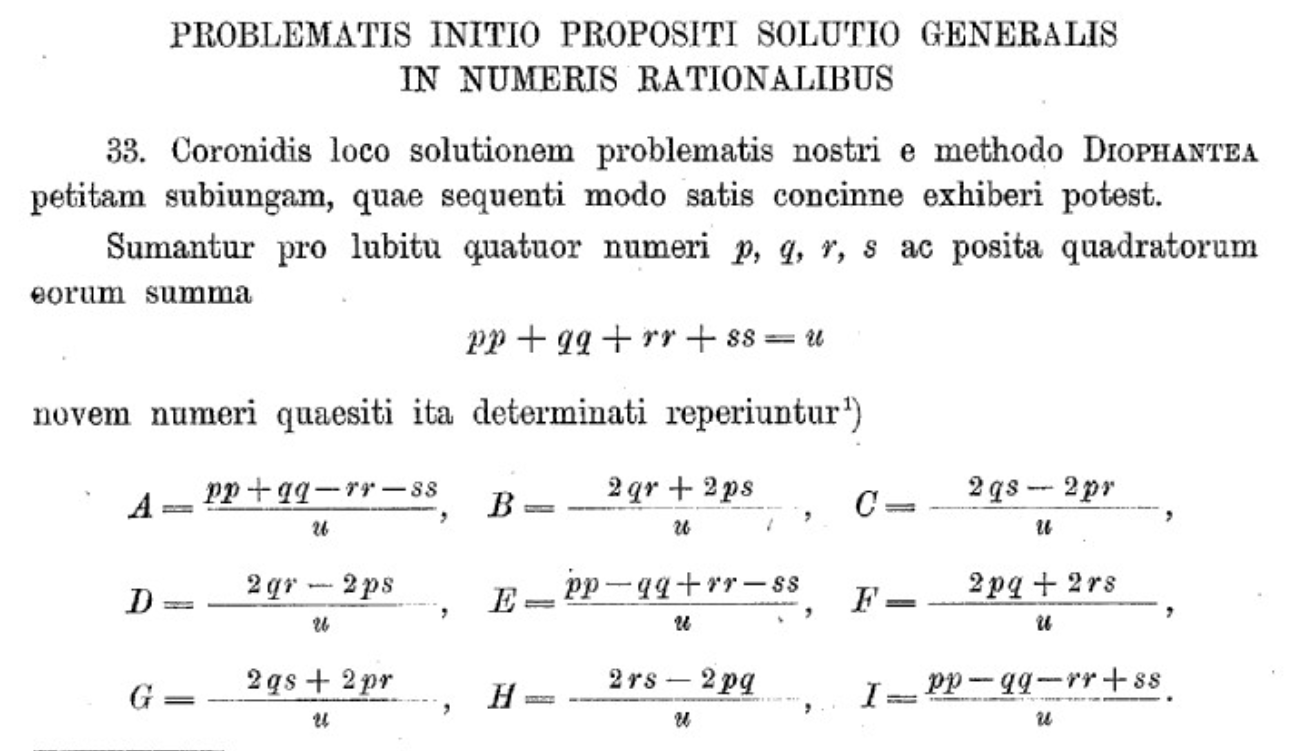
\includegraphics[width=5cm]{Euler}
    \caption{Euler's representation of rotations}
\end{figure}

\end{frame}

\section{Proof in Coq}

\begin{frame}[fragile]
\frametitle{Representing Groups}
\begin{itemize}
	\item groups are represented as a \textit{typeclass}
	\item essentially a typeclass is a dependently-typed record, with some extra type inference capabilities
	\item a subtle point is that this allows \textit{different equivalence relations}
\end{itemize}

\begin{lstlisting}[language=Coq]
Class Group := {
        id : G
      ; inverse: G -> G
      ; rel_equiv: equiv G Grel
      ; id_left: forall x: G, (id • x) •= x
      ; id_right: forall x: G, (x • id) •= x
      ; assoc: forall x y z: G, (x • y) • z •= x • (y • z)
      ; right_inv: forall x: G, x • (inverse x) •= id
}.
\end{lstlisting}
\end{frame}

\begin{frame}[fragile]
\frametitle{Representing Morphisms}

Likewise, homomorphism and isomorphism can be represented with typeclasses

\begin{lstlisting}[language=Coq]{Name}
Class GroupHomomorphism G H
  (Gop: G -> G -> G) 
  (Hop: H -> H -> H) 
  (Grel: relation G)
  (Hrel: relation H)
  (hom_f: G -> H)
: Type 
:= {
    hom_left_group: Group G Gop Grel
  ; hom_right_group: Group H Hop Hrel
  ; hom_mul {a1 a2}: Hrel
                      (hom_f (Gop a1 a2)) 
                      (Hop (hom_f a1) (hom_f a2))
}.
\end{lstlisting}

\end{frame}


\begin{frame}[fragile]
\frametitle{Representing Morphisms}

Another subtle point about having multiple equivalence relations is that we must prove they are ``compatible"

\begin{lstlisting}[language=Coq, basicstyle=\tiny]{Name}
Section hom_trans.
Variables A B C : Type.

Variable Arel: relation A.
Variable Brel: relation B.
Variable Crel: relation C.

Variable A_Eq: Equivalence Arel.
Variable B_Eq: Equivalence Brel.
Variable C_Eq: Equivalence Crel.

Variable AtoB: A -> B.
Variable BtoC: B -> C.

Variables Aop: A -> A -> A.
Variables Bop: B -> B -> B.
Variables Cop: C -> C -> C.

Variable BtoC_rw   : Proper (Brel ≈ Crel) BtoC.

Lemma GroupHomomorphism_trans:
  GroupHomomorphism A B Aop Bop Arel Brel AtoB ->
  GroupHomomorphism B C Bop Cop Brel Crel BtoC ->
  GroupHomomorphism A C Aop Cop Arel Crel (fun a => BtoC (AtoB a)).
Proof.
...
\end{lstlisting}

\end{frame}

\begin{frame}[fragile]
\frametitle{Representing Matrices, complex numbers, and quaternions}

\begin{itemize}
	\item we can represent groups abstractly, but it somewhat interesting to directly work with the underlying types
	\item complex numbers and quaternions are represented as pairs of real numbers
	\item a matrix is represented as a function that takes two natural numbers and returns a complex number
\end{itemize}

\begin{lstlisting}[language=Coq]
Definition C := (R * R)%type

Definition Quaternion := (R * R * R * R)%type.

Definition Matrix (m n : nat) := nat -> nat -> C.
\end{lstlisting}
\end{frame}


\begin{frame}[fragile]
\frametitle{Subset Types}

\begin{itemize}
	\item \textit{Subset types} carry both a value and a proof that the values satisfies some predicate
	\item any function involving these types also carries a proof of closure
\end{itemize}

\begin{lstlisting}[language=Coq]
Definition Versor := { q | Qnorm q = 1}.

Definition SU2 := { 
	U: Matrix 2 2
  | WF_Matrix U /\                                                                               
    (U 0 0 = Cconj (U 1 1) /\ U 0 1 = - Cconj (U 1 0) ) /\
    d2_det U = C1 }.

Definition SO3 := { 
	U: Matrix 3 3 
	| WF_Matrix U /\ Real_matrix U /\ 
		U × (U) ⊤ ≡ I 3 /\ (U) ⊤ × U ≡ I 3 /\ 
		d3_det U = C1 }. 
\end{lstlisting}
\end{frame}

\begin{frame}[fragile]
\frametitle{Subset Types}
\begin{lstlisting}[language=Coq, basicstyle=\tiny]
Definition Versor_to_SU2 (v: Versor): SU2.    
Proof.    
  destruct v as [(((x, y), z), w) E].    
  unfold SU2.    
  exists (    
    fun row => fun col =>    
    match row, col with    
    | 0, 0 => (x, y)    
    | 0, 1 => (z, w)    
    | 1, 0 => (Ropp z, w)    
    | 1, 1 => (x, Ropp y)    
    | _, _ => C0    
    end    
  ).    
  unfold Qnorm in E.    
  apply pow_eq with (n := 2%nat) in E.    
  rewrite pow2_sqrt in E.    
  replace ((1^2)%R) with 1 in E by lra.    
  repeat split.    
  - show_wf.    
  - lca.    
  - lca.    
  - unfold d2_det, Cmult, Cminus, Cplus, C1.    
     simpl. f_equal.    
     rewrite <- E.    
     all: lra.    
  - repeat apply Rplus_le_le_0_compat.    
     all: apply pow2_ge_0.    
Defined.
\end{lstlisting}
\end{frame}


\begin{frame}[fragile]
\frametitle{Subset Types}
\begin{itemize}
	\item I define equality of these subset types as equality of their values (first projection)
	\item this is general, as this also takes an equivalence relation
\end{itemize}

\begin{lstlisting}[language=Coq]
Definition sigma_proj1_rel
  {X: Type} 
  {A: X -> Prop} 
  {rel: relation X}
  (e: Equivalence rel)
  (s1 s2: sig A) 
  : Prop 
:= rel (proj1_sig s1) (proj1_sig s2).
\end{lstlisting}
\end{frame}

\begin{frame}[fragile]
\frametitle{SU(2) $\to$ SO(3)}
\begin{lstlisting}[language=Coq, basicstyle=\tiny]
Theorem SU2_Homomorphism_SO3:
  GroupHomomorphism
    SU2
    SO3
    SU2_mul
    SO3_mul
    SU2_equiv
    SO3_equiv
    (fun U => Versor_to_SO3 (SU2_to_Versor U)).
Proof.
  apply GroupHomomorphism_trans with versor_equiv Vmul.
  - apply (sigma_proj1_rel_equivalence eq_equivalence).
  - apply (sigma_proj1_rel_equivalence mat_equiv_equivalence).
  - unfold Morphisms.Proper, Morphisms.respectful.
    intros.
    unfold versor_equiv, SO3_equiv, sigma_proj1_rel, proj1_sig in *.
    destruct x as [(((a1, b1), c1), d1) E1].
    destruct y as [(((a2, b2), c2), d2) E2].
    by_cell; inversion H; subst; reflexivity.
  - apply SU2_Iso_to_hom.
  - apply Versor_Homomorphism_SO3.
Qed.
\end{lstlisting}
\end{frame}

\section{Q\&A}

\begin{frame}[c]
\begin{center}
\Huge Questions?
\end{center}
\end{frame}

\begin{frame}[allowframebreaks]
        \frametitle{References}
        \bibliographystyle{amsalpha}
        \bibliography{references.bib}
\end{frame}

\end{document}
